\documentclass{article}
\usepackage[utf8]{inputenc}
\usepackage{amsmath}
\usepackage[onehalfspacing]{setspace}
\usepackage{tikz}
\usepackage{pgfplots}

\pagenumbering{gobble}

\pgfplotsset{
    compat = 1.15,
    common grid/.style = {
        grid = both,
        grid style = {
            line width = 0.1pt,
            draw = gray!10
        },
        major grid style = {
            line width = 0.2pt,
            draw = gray!50
        },
        minor tick num = 5
    }
}

\begin{document}

\begin{figure}[hbt!]
    \centering
    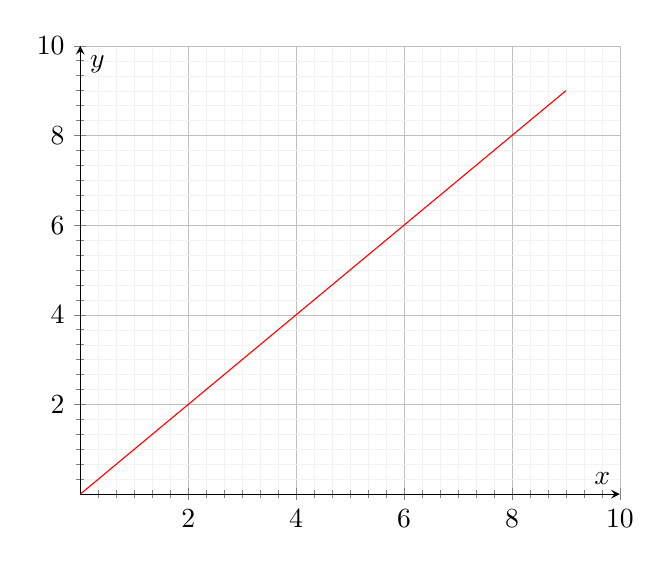
\begin{tikzpicture}
        \begin{axis}[
            axis lines = middle,
            ylabel = $y$,
            xlabel = $x$,
            xmin = 0,
            xmax = 10,
            ymin = 0,
            ymax = 10,
            common grid]
            \addplot [
                samples = 2,
                domain = 0:9,
                color=red] {x};
        \end{axis}
    \end{tikzpicture}
    \caption{Graph of \ref{eq:1}$^{st}$ equation}
\end{figure}

\begin{equation}
    \label{eq:1}
    f(x) = x
\end{equation}

\begin{figure}[hbt!]
    \centering
    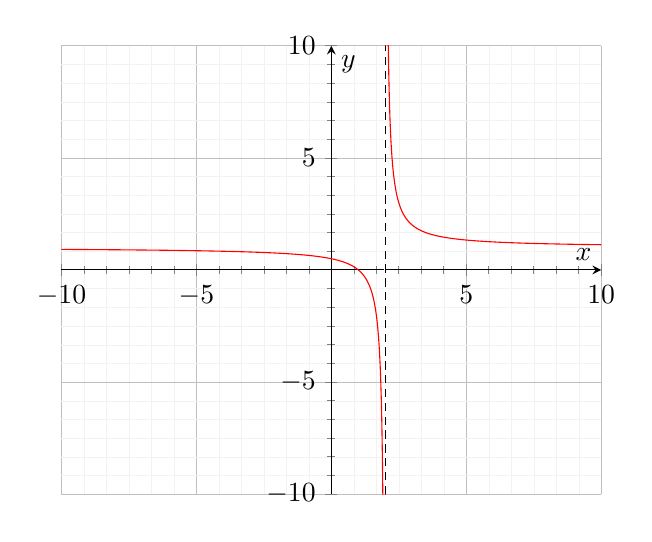
\begin{tikzpicture}
        \begin{axis}[
            axis lines = middle,
            ylabel = $y$,
            xlabel = $x$,
            ymin = -10,
            ymax = 10,
            xmin =- 10,
            xmax = 10,
            common grid]
            \addplot [
                samples = 1000,
                domain = -10:10,
                color=red] {(x-1)/(x-2)};

            % hide line that connects graph
            \draw [thick, white] ({rel axis cs:0,0} -| {axis cs:2,0}) -- ({rel axis cs:0,1} -| {axis cs:2,0.1});
            % draw vertical asymptote
            \draw [densely dashed] ({rel axis cs:0,0} -| {axis cs:2,0}) -- ({rel axis cs:0,1} -| {axis cs:2,0});
        \end{axis}
    \end{tikzpicture}
    \caption{Graph of \ref{eq:2}$^{nd}$ equation}
\end{figure}

\begin{equation}
    \label{eq:2}
    f(x) = \frac{x-1}{x-2}
\end{equation}

\end{document}